\documentclass[a4paper, 10pt, final, garamond]{book}
\usepackage{cours-preambule}
\usepackage[french]{babel}

\raggedbottom

\makeatletter
\renewcommand{\@chapapp}{Induction -- chapitres}
\renewcommand\thechapter{1 et 2}
\makeatother

\begin{document}
% \setcounter{chapter}{2}

\chapter{TD~: Champ magnétique et ses actions mécaniques}

\section{Aimant en U}
\label{sec:exaimu}
\noindent
\begin{minipage}[t]{.5\linewidth}
  On donne la carte de champ d'un aimant en U.
  \bigbreak
  \begin{enumerate}
    \item Donner l'emplacement des pôles, les zones de champ fort et faible.
    \item Indiquer la zone où le champ est uniforme.
    \item Préciser la direction du champ magnétique dans l'entrefer.
    \item Donner deux autres moyens de créer un champ uniforme.
  \end{enumerate}
\end{minipage}
\begin{minipage}[t]{.5\linewidth}
  ~
  \vspace*{-10pt}
  \begin{center}
    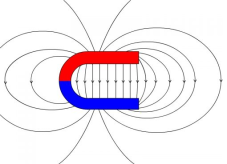
\includegraphics[scale=.8]{exaimu}
    \label{fig:exaimu}
  \end{center}
\end{minipage}

\section{Cartes de champ}
\label{sec:excchp}
Dans les cartes de champ magnétique suivantes, où le champ est-il le plus
intense~? Où sont placées les spires à l'origine de ces champs~? Indiquer pour
chacune le sens de parcours du courant.
\begin{figure}[h]
  \centering
  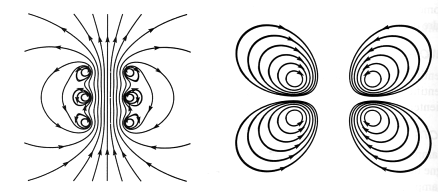
\includegraphics[scale=1]{cchp}
  \label{fig:excchp}
\end{figure}

\section{Aimantation d'un matériau}
\label{sec:aimat}
\noindent
\begin{minipage}[c]{.4\linewidth}
  \label{tab:aimat}
  \begin{center}
    \begin{tabular}[c]{lc}
      \toprule
      Matériau & Aimantation (\si{kA.m^{-1}})
      \\\midrule
      \ce{AlNiCo} 200 & \num{600}
      \\
      Ferrite 1000 & \num{1700}
      \\
      \ce{NdFeB} & \num{3000}
      \\
      \ce{SmCo} 17 & \num{4000}
      \\\bottomrule
    \end{tabular}
  \end{center}
\end{minipage}
\hfill
\noindent
\begin{minipage}[c]{.55\linewidth}
  % \vspace*{3pt}
  Le tableau ci-contre indique les ordres de grandeur d'aimantation de plusieurs
  matériaux magnétiques permettant de fabriquer des aimants permanents.
  L'aimantation d'un matériau est définie comme le \textbf{moment magnétique
  volumique}, c'est-à-dire le moment magnétique d'un échantillon de ce matériau
  divisé par son volume.
\end{minipage}
\bigbreak
\begin{enumerate}
  \item Rappeler la dimension d'un moment magnétique, et vérifier l'unité de
    l'aimantation donnée dans le tableau.
  \item Les matériaux pour fabriquer des aimants permanents doivent-ils posséder
    une aimantation forte ou faible ?
  \item Considérons un aimant cylindrique \ce{NdFeB} (néodyme, fer, bore),
    d'épaisseur $e = \SI{1}{mm}$ et de rayon $R = \SI{5}{mm}$. Calculer son
    moment magnétique.
  \item Combien de spires de même rayon $R$ et parcourues par un courant
    d’intensité $I = \SI{100}{mA}$ faudrait-il bobiner pour obtenir le même
    moment magnétique ?
\end{enumerate}

\section{Équilibre d'un aimant}
\label{sec:exeqaim}
\noindent
\begin{minipage}[t]{.7\linewidth}
  Un aimant très fin, de moment magnétique $\vv{\mu}$ et de masse $m$, repose en
  équilibre sur une pointe en O. Il est soumis à l'action d'un champ magnétique
  uniforme $\vv{B}$ et au champ de pesanteur terrestre $\vv{g}$. On appelle G le
  centre d'inertie de l'aimant.
  \smallbreak
  Exprimer la distance $d = \rm OG$ pour que l'aimant reste en équilibre
  horizontal.
\end{minipage}
\hfill
\begin{minipage}[t]{.3\linewidth}
  ~
  \vspace*{-20pt}
  \begin{center}
    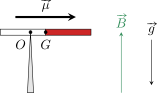
\includegraphics[scale=1]{exeqaim}
    \label{fig:exeqaim}
  \end{center}
\end{minipage}

\section{Rails de \textsc{Laplace} inclinés}
\label{sec:railpl}
On reprend les rails de \textsc{Laplace}, mais en les inclinant~: au lieu d'être
horizontaux, ils forment un angle $\alpha = \ang{30;;}$ avec la verticale. Le
champ magnétique est supposé stationnaire, uniforme, vertical dirigé vers le
haut, de norme \SI{150}{mT}. Le barreau mobile des rails de \textsc{Laplace}
pèse \SI{8.0}{kg} et est long de $\ell = \SI{12}{cm}$. Les frottements sont
négligés, de même que tout phénomène d'induction.
\begin{enumerate}
  \item Faire un schéma du dispositif en représentant les différentes forces
    agissant sur le barreau mobile. Quel doit être le sens du courant dans le
    circuit pour que la force de \textsc{Laplace} retienne le barreau~?
  \item Déterminer l'intensité du courant permettant l'équilibre du barreau.
  \item Partant de cette situation, on communique au barreau une vitesse
    initiale $v_0$ dirigée vers le haut. Déterminer son mouvement ultérieur.
  \item En raisonnant à partir de la loi de \textsc{Lenz} (chapitre suivant),
    indiquer qualitativement comment est modifiée la réponse à la question
    précédente lorsque l'on tient compte de l'induction.
\end{enumerate}

\section{Mesure du champ magnétique terrestre}
\label{sec:meschpterre}
Dans un laboratoire situé à Paris, on souhaite déterminer la norme
$\norm{\vv{B}_h}$ de la composante horizontale locale $\vv{B}_h$ (dont le sens
et la direction sont donnés sur la Figure~\ref{fig:magTsens}) grâce à un
dispositif d'\textsc{Œrsted} (Figure~\ref{fig:orsted}). Ce dernier est constitué
d'une aiguille aimantée libre de pivoter sans frottement sur son axe, fixé à un
socle transparent et un fil de cuivre relié à deux bornes de sécurité fixées au
même socle transparent, de courant admissible \SI{5}{A}.
\noindent
\begin{minipage}[t]{.5\linewidth}
  \begin{center}
    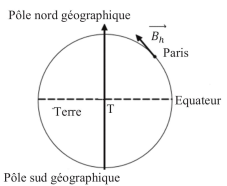
\includegraphics[scale=1]{magTsens}
    \captionof{figure}{Sens de la composante horizontale locale du champ
    magnétique terrestre à Taris.}
    \label{fig:magTsens}
  \end{center}
\end{minipage}
\hfill
\begin{minipage}[t]{.5\linewidth}
  \begin{center}
    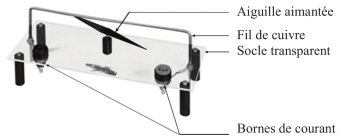
\includegraphics[scale=1]{orsted}
    \captionof{figure}{Dispositif d'\textsc{Œrsted}}
    \label{fig:orsted}
  \end{center}
\end{minipage}
\begin{rexem}{Matériel}
  \noindent
  \begin{minipage}[t]{.5\linewidth}
    \begin{itemize}[label=$\diamond$, leftmargin=10pt]
      \item un rapporteur~;
      \item des files électriques~;
      \item un interrupteur~;
    \end{itemize}
  \end{minipage}
  \hfill
  \begin{minipage}[t]{.5\linewidth}
    \begin{itemize}[label=$\diamond$, leftmargin=10pt]
      \item une alimentation électrique stabilisée \SIrange{0}{30}{V}/\SI{5}{A}~;
      \item un ampèremètre~;
      \item un teslamètre permettant la mesure d'intensité de champs
        magnétiques entre \SIrange{0.1}{100}{mT}.
    \end{itemize}
  \end{minipage}
\end{rexem}
\begin{tdefi}{Donnée}
  Le champ magnétique créé par un fil infini parcouru par un courant $I$
  s'exprime, dans un système de coordonnées cylindriques d'axe $z$ orienté par
  le sens réel du courant, par~:
  \[
    \vv{B} = \frac{\mu_0 I}{2\pi r}\ut
  \]
  avec $\mu_0 = 4\pi \cdot \SI{e-7}{H.m^{-1}}$. On admet que le champ créé par
  le fil du dispositif d'\textsc{Œrsted} est convenablement décrit par cette
  expression.
\end{tdefi}
On souhaite établir un protocole permettant de mesurer la composante horizontale
locale du champ magnétique terrestre à Paris en exploitant le principe de
superposition des champs magnétiques.
\begin{enumerate}
  \item Pour quelle raison ne peut-on pas se servir directement du teslamètre
    pour effectuer la mesure~?
  \item On suppose que le fil est parcouru par un courant d'intensité $I =
    \SI{1}{A}$. Calculer la valeur du champ magnétique à $r = \SI{2}{cm}$ du
    fil.
  \item Décrire et schématiser l'expérience à réaliser en vous servant du
    matériel mis à votre disposition, exception faite du teslamètre.
  \item Préciser les mesures à réaliser, et la technique numérique à employer
    pour trouver la valeur.
  \item Donner un ordre de grandeur des grandeurs physiques à employer pour
    réaliser l'expérience.
\end{enumerate}

\end{document}
